% Options for packages loaded elsewhere
\PassOptionsToPackage{unicode}{hyperref}
\PassOptionsToPackage{hyphens}{url}
%
\documentclass[
  a4paper,
]{scrbook}

\usepackage{amsmath,amssymb}
\usepackage{lmodern}
\usepackage{iftex}
\ifPDFTeX
  \usepackage[T1]{fontenc}
  \usepackage[utf8]{inputenc}
  \usepackage{textcomp} % provide euro and other symbols
\else % if luatex or xetex
  \usepackage{unicode-math}
  \defaultfontfeatures{Scale=MatchLowercase}
  \defaultfontfeatures[\rmfamily]{Ligatures=TeX,Scale=1}
  \setmainfont[]{Latin Modern Roman}
  \setsansfont[]{Latin Modern Roman}
\fi
% Use upquote if available, for straight quotes in verbatim environments
\IfFileExists{upquote.sty}{\usepackage{upquote}}{}
\IfFileExists{microtype.sty}{% use microtype if available
  \usepackage[]{microtype}
  \UseMicrotypeSet[protrusion]{basicmath} % disable protrusion for tt fonts
}{}
\makeatletter
\@ifundefined{KOMAClassName}{% if non-KOMA class
  \IfFileExists{parskip.sty}{%
    \usepackage{parskip}
  }{% else
    \setlength{\parindent}{0pt}
    \setlength{\parskip}{6pt plus 2pt minus 1pt}}
}{% if KOMA class
  \KOMAoptions{parskip=half}}
\makeatother
\usepackage{xcolor}
\setlength{\emergencystretch}{3em} % prevent overfull lines
\setcounter{secnumdepth}{5}
% Make \paragraph and \subparagraph free-standing
\ifx\paragraph\undefined\else
  \let\oldparagraph\paragraph
  \renewcommand{\paragraph}[1]{\oldparagraph{#1}\mbox{}}
\fi
\ifx\subparagraph\undefined\else
  \let\oldsubparagraph\subparagraph
  \renewcommand{\subparagraph}[1]{\oldsubparagraph{#1}\mbox{}}
\fi


\providecommand{\tightlist}{%
  \setlength{\itemsep}{0pt}\setlength{\parskip}{0pt}}\usepackage{longtable,booktabs,array}
\usepackage{calc} % for calculating minipage widths
% Correct order of tables after \paragraph or \subparagraph
\usepackage{etoolbox}
\makeatletter
\patchcmd\longtable{\par}{\if@noskipsec\mbox{}\fi\par}{}{}
\makeatother
% Allow footnotes in longtable head/foot
\IfFileExists{footnotehyper.sty}{\usepackage{footnotehyper}}{\usepackage{footnote}}
\makesavenoteenv{longtable}
\usepackage{graphicx}
\makeatletter
\def\maxwidth{\ifdim\Gin@nat@width>\linewidth\linewidth\else\Gin@nat@width\fi}
\def\maxheight{\ifdim\Gin@nat@height>\textheight\textheight\else\Gin@nat@height\fi}
\makeatother
% Scale images if necessary, so that they will not overflow the page
% margins by default, and it is still possible to overwrite the defaults
% using explicit options in \includegraphics[width, height, ...]{}
\setkeys{Gin}{width=\maxwidth,height=\maxheight,keepaspectratio}
% Set default figure placement to htbp
\makeatletter
\def\fps@figure{htbp}
\makeatother

\usepackage{titling}
\setlength{\droptitle}{-2cm}
\preauthor{
  \begin{center}
  \Large
  \vspace{10mm}
  by

  \vspace{20mm}
}
\postauthor{
  \end{center}
  \vfill
}

\predate{
  \begin{center}
  A thesis 
  submitted in fulfilment of the \\
  requirements of the degree of \\
  Doctor of Philosophy in Physics\\               % Degree
  School of Physical and Chemical Sciences\\          % Department
  Te Herenga Waka - Victoria University of Wellington\\                       % University 
  \vspace{5mm}
}
\postdate{
  \\
  
\includegraphics[width=3in,height=1.5in]{figures/VUW-logo.png}\\
  \end{center}
  }
\makeatletter
\makeatother
\makeatletter
\@ifpackageloaded{bookmark}{}{\usepackage{bookmark}}
\makeatother
\makeatletter
\@ifpackageloaded{caption}{}{\usepackage{caption}}
\AtBeginDocument{%
\ifdefined\contentsname
  \renewcommand*\contentsname{Table of contents}
\else
  \newcommand\contentsname{Table of contents}
\fi
\ifdefined\listfigurename
  \renewcommand*\listfigurename{List of Figures}
\else
  \newcommand\listfigurename{List of Figures}
\fi
\ifdefined\listtablename
  \renewcommand*\listtablename{List of Tables}
\else
  \newcommand\listtablename{List of Tables}
\fi
\ifdefined\figurename
  \renewcommand*\figurename{Figure}
\else
  \newcommand\figurename{Figure}
\fi
\ifdefined\tablename
  \renewcommand*\tablename{Table}
\else
  \newcommand\tablename{Table}
\fi
}
\@ifpackageloaded{float}{}{\usepackage{float}}
\floatstyle{ruled}
\@ifundefined{c@chapter}{\newfloat{codelisting}{h}{lop}}{\newfloat{codelisting}{h}{lop}[chapter]}
\floatname{codelisting}{Listing}
\newcommand*\listoflistings{\listof{codelisting}{List of Listings}}
\makeatother
\makeatletter
\@ifpackageloaded{caption}{}{\usepackage{caption}}
\@ifpackageloaded{subcaption}{}{\usepackage{subcaption}}
\makeatother
\makeatletter
\@ifpackageloaded{tcolorbox}{}{\usepackage[many]{tcolorbox}}
\makeatother
\makeatletter
\@ifundefined{shadecolor}{\definecolor{shadecolor}{rgb}{.97, .97, .97}}
\makeatother
\makeatletter
\makeatother
\ifLuaTeX
  \usepackage{selnolig}  % disable illegal ligatures
\fi
\usepackage[citestyle = ieee,urldate = iso8601]{biblatex}
\addbibresource{references.bib}
\IfFileExists{bookmark.sty}{\usepackage{bookmark}}{\usepackage{hyperref}}
\IfFileExists{xurl.sty}{\usepackage{xurl}}{} % add URL line breaks if available
\urlstyle{same} % disable monospaced font for URLs
\hypersetup{
  pdftitle={Volatile Organic Compound Detection Using Insect Odorant-Receptor Functionalised Field-Effect Transistors},
  pdfauthor={Eddyn Oswald Perkins Treacher},
  hidelinks,
  pdfcreator={LaTeX via pandoc}}

\title{Volatile Organic Compound Detection Using Insect Odorant-Receptor
Functionalised Field-Effect Transistors}
\author{Eddyn Oswald Perkins Treacher}
\date{Aug 2023}

\begin{document}
\frontmatter
\maketitle
\ifdefined\Shaded\renewenvironment{Shaded}{\begin{tcolorbox}[frame hidden, boxrule=0pt, breakable, interior hidden, borderline west={3pt}{0pt}{shadecolor}, sharp corners, enhanced]}{\end{tcolorbox}}\fi

\mainmatter
\bookmarksetup{startatroot}

\hypertarget{acknowledgements}{%
\chapter*{Acknowledgements}\label{acknowledgements}}
\addcontentsline{toc}{chapter}{Acknowledgements}

\markboth{Acknowledgements}{Acknowledgements}

Thanks for all the fish.

\bookmarksetup{startatroot}

\hypertarget{abstract}{%
\chapter*{Abstract}\label{abstract}}
\addcontentsline{toc}{chapter}{Abstract}

\markboth{Abstract}{Abstract}

This is a thesis skeleton written with quarto. Make a copy of this
thesis repo and start to write!

Make a new paragraph by leaving a blank line.

\newpage
\tableofcontents

\bookmarksetup{startatroot}

\hypertarget{introduction}{%
\chapter{Introduction}\label{introduction}}

This is a book created from markdown and executable code.

See for additional discussion of literate programming.

\begin{verbatim}
[1] 2
\end{verbatim}

\bookmarksetup{startatroot}

\hypertarget{carbon-nanotube-and-graphene-field-effect-transistors}{%
\chapter{Carbon Nanotube and Graphene Field-Effect
Transistors}\label{carbon-nanotube-and-graphene-field-effect-transistors}}

\hypertarget{device-functionalisation}{%
\section{Device Functionalisation}\label{device-functionalisation}}

\hypertarget{insect-odorant-receptors}{%
\section{Insect Odorant Receptors}\label{insect-odorant-receptors}}

\bookmarksetup{startatroot}

\hypertarget{carbon-nanotube-and-graphene-field-effect-transistors-as-biosensor-platforms}{%
\chapter{Carbon Nanotube and Graphene Field-Effect Transistors as
Biosensor
Platforms}\label{carbon-nanotube-and-graphene-field-effect-transistors-as-biosensor-platforms}}

\bookmarksetup{startatroot}

\hypertarget{sec-fabrication}{%
\chapter{Fabrication of Carbon Nanotube Network and Graphene
Field-Effect Transistors}\label{sec-fabrication}}

This chapter discusses the fabrication processes for both the carbon
nanotube network and graphene transistors. Experimental optimisation of
the transducer element is critical for biosensor work, and large numbers
of transducers were required for testing various biosensor
functionalisation processes. Therefore, these processes were developed
to rapidly fabricate devices with reproducible device characteristics
appropriate for biosensing work. Also outlined in this chapter are the
characterisation techniques taken to test the quality and
reproducibility of these fabrication processes.

The nitrogen (\(\geq\) 99.99\%) and oxygen (99.7\%) used in fabrication
work was supplied by BOC Limited New Zealand. Deionised (DI) water was
taken from a Synergy\(^\circledR\) UV Water Purification System. The DI
water had a measured conductivity of
\((1.4\pm0.1)\textrm{ } \mu \textrm{S cm}^{-1}\), compared to tap water
with a measured conductivity of
\((7.8\pm0.2)\textrm{ } \mu \textrm{S cm}^{-1}\).

\hypertarget{sec-dep-carbon-nanotubes}{%
\section{Deposition of Carbon
Nanotubes}\label{sec-dep-carbon-nanotubes}}

4-inch \(p\)-type (B-doped) silicon wafers with either a 100 nm or 300
nm SiO\(_2\) layer (WaferPro LLC) were used as the substrate for carbon
nanotube network deposition. A 100 nm SiO\(_2\) layer was the preferred
option for the devices intended for backgated measurements. Before
deposition of carbon nanotubes, the wafers were spin-coated with
AZ\(^\circledR\) 1518 photoresist, placed photoresist-side down onto a
cleanroom wipe, fixed in place using vacuum suction, then cleaved into
quarters using a diamond-tipped scribe tool. For fabrication performed
before June 2023, the protective photoresist layer was then removed by
soaking the quarter-wafers in acetone for 15 minutes, then rinsed with
isopropyl alcohol (IPA) and dried with N\(_2\) gas. However, for
complete removal of photoresist, we found it was necessary to flood
expose the wafer with the Karl Suss Aligner for 1 min and then place it
in AZ326 developer for 3 min, as discussed further in
Section~\ref{sec-fluorescence-characterisation}.

Carbon nanotubes were deposited before alignment markers
photolithography on all wafers fabricated between Aug 2021-Feb 2023,
while devices fabricated before Aug 2021 and after Feb 2023 had
alignment markers photolithography performed before the deposition of
carbon nanotubes. The process order was first switched in Aug 2021 as
this order led to faster processing times. However, the order was
switched back in Feb 2023 to minimise the exposure of carbon nanotubes
to photolithographic chemical processes.

\hypertarget{solvent-based}{%
\subsection{Solvent-Based}\label{solvent-based}}

The solvent-based deposition process for the carbon nanotube network in
the second fabrication protocol is as follows. 10 mg of
2-mercaptopyridine (99\%, Sigma-Aldrich) was dissolved in 1 ml ethanol
by sonication until clear. Quarter wafers were sonicated in acetone for
3 min, then exposed to O\(_2\) plasma at 100 W for at least 2 min in a
small plasma cleaner (Plasma Etch, Inc., PE-50 Compact Benchtop Plasma
Cleaning System) or reactive ion etcher (Oxford Instruments,
Plasmalab\(^\circledR\) 80 Plus) under 300 mTorr pressure. The cleaned
SiO\(_2\)/Si surface was then coated with 2-mercaptopyridine for 10
minutes, rinsed with ethanol to remove residual \(2\)-mercaptopyridine,
and then nitrogen dried. Meanwhile, 5 \(\mu\) g of 99\% semiconducting
carbon nanotube bucky paper (NanoIntegris, IsoNanotubes S-99) was
dispersed in 10 mL of anhydrous 1,2-dichlorobenzene (Sigma Aldrich) by
ultrasonication until no particles were visible to the naked eye. During
this time, the ultrasonic bath temperature was kept between 20 - 30
\(^\circ\)C or the buckypaper would not disperse successfully. The
substrates were then placed into a dish with CNT-DCB suspension and left
covered for 1 hour, dipped into ethanol for 10 min to remove residual
solvent and any unattached carbon nanotube bundles, and then dried with
nitrogen.

\hypertarget{surfactant-based}{%
\subsection{Surfactant-Based}\label{surfactant-based}}

Two different approaches were used to attach the surfactant-dispersed
CNTs. In both approaches, the quarter wafers were rinsed with ultrapure
deionised water (DI water), acetone and IPA before being placed into a
reactive ion etcher (Oxford Instruments, Plasmalab 80 Plus) and exposed
to O\(_2\) plasma at 100 W for at least 2 min in a small plasma cleaner
(Plasma Etch, Inc, PE-50 Compact Benchtop Plasma Cleaning System) or
reactive ion etcher (Oxford Instruments, Plasmalab 80 Plus) under 300
mTorr pressure to make the surface hydrophilic. 1 mL of poly-L-lysine
(PLL) was immediately deposited onto each quarter wafer and left for 5
minutes. Then, the quarter wafers were rinsed for 30 s with DI water and
dried with N\(_2\) gas. This process allows for the surface adhesion of
semiconducting single carbon nanotubes suspended in surfactant.

\hypertarget{simple-dropcasting}{%
\subsubsection*{Simple Dropcasting}\label{simple-dropcasting}}
\addcontentsline{toc}{subsubsection}{Simple Dropcasting}

2 mL of IsoNanotubes-S 90\% or 99\% solution (NanoIntegris) was decanted
into a small bottle and sonicated for 5 s to break up bundles of CNTs.
An even spread of 400 \(\mu\)L CNT solution was placed in the centre of
the PLL-functionalised quarter wafer, covered and left for 10 minutes.
The CNT solution was then rinsed off with DI water and IPA, and then the
quarter wafer was dried with N\(_2\) gas. Next, the quarter wafer was
annealed in a vacuum oven at 150\(^\circ\) C for 1 hour. This method
would often lead to an inhomogeneous spread of CNTs across the quarter
wafer surface, detailed further in section
Section~\ref{sec-AFM-characterisation}.

\hypertarget{steam-assisted-method}{%
\subsubsection*{Steam-Assisted Method}\label{steam-assisted-method}}
\addcontentsline{toc}{subsubsection}{Steam-Assisted Method}

2 mL of IsoNanotubes-S 90\% or 99\% solution (NanoIntegris) was decanted
into a small bottle and burst-sonicated once (on then off again) to
break up bundles of CNTs. 75 mL of 95\(^\circ\) C water was then placed
into a glass dish on a hotplate held at 95\(^\circ\) C. After this, the
PLL-functionalised quarter wafer was placed in the centre of an
insulating surface on the same hotplate. The CNT dispersion was
carefully spread across the surface of the wafer without spilling any
over the wafer edges. The wafer on the insulating surface and glass dish
were then left under the same cover for 2 minutes to expose the wafer to
steam from the glass dish. The use of an insulating surface meant that
the wafer and CNT dispersion were not heated from below while exposed to
steam. The CNT dispersion was then rinsed off the wafer with DI water,
ethanol, acetone and IPA, and then the quarter wafer was dried with
N\(_2\) gas. As in the original method, the quarter wafer was then
annealed in a vacuum oven at 150\(^\circ\) C for 1 hour. This method
gave an even spread of CNTs across the quarter wafer surface, leading to
a greater consistency in performance between devices. Further details
can be found in section Section~\ref{sec-AFM-characterisation}.

\hypertarget{photolithography-for-carbon-nanotube-and-graphene-field-effect-transistors}{%
\section{Photolithography for Carbon Nanotube and Graphene Field-Effect
Transistors}\label{photolithography-for-carbon-nanotube-and-graphene-field-effect-transistors}}

\begin{figure}

{\centering 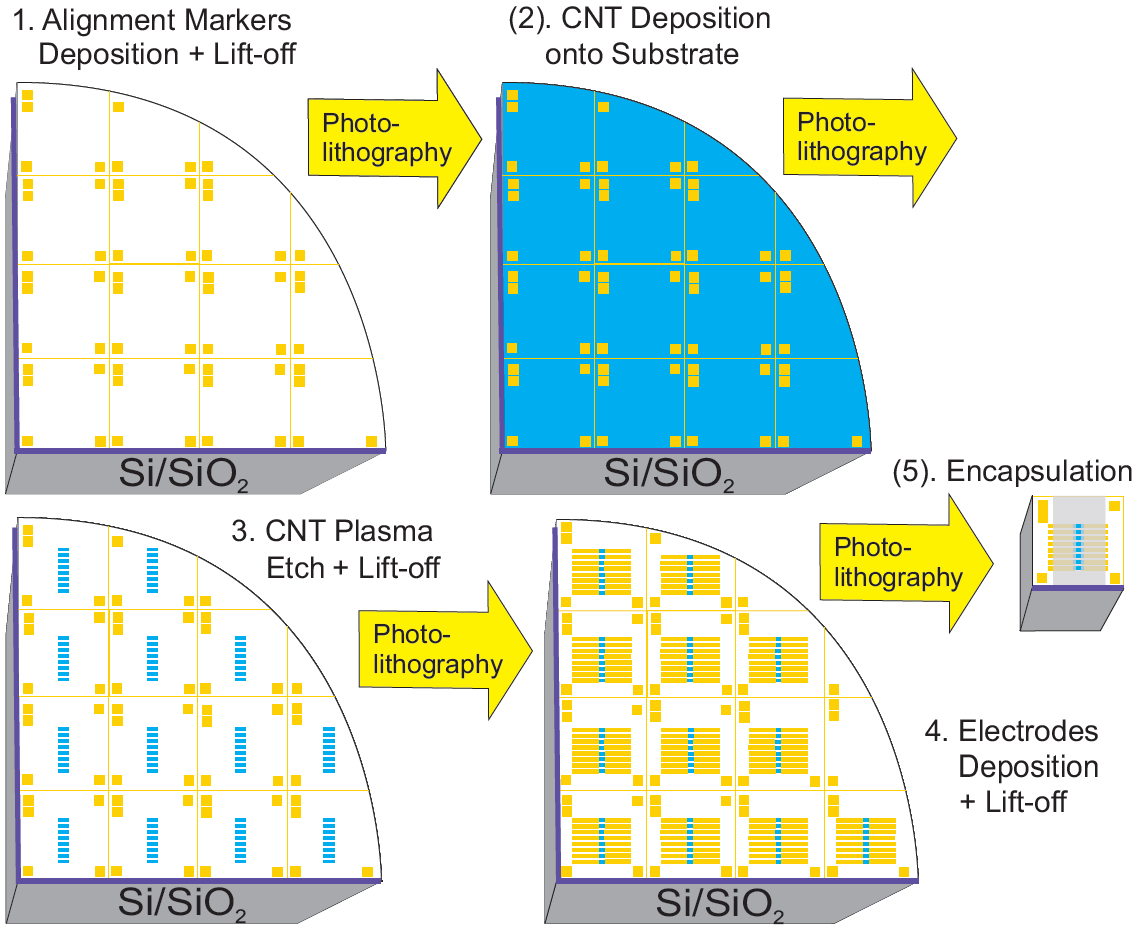
\includegraphics[width=0.9\textwidth,height=\textheight]{./figures/ch4/photolithography-cycle.png}

}

\caption{\label{fig-qw-photolithography}The photolithographic processes
used for fabrication of both carbon nanotube and graphene devices
(graphene devices were fabricated individually for every step, step \#2
skipped for graphene devices)}

\end{figure}

Photolithography was used to define eight channel regions on each device
and subsequently to define metal contacts for each of these channels. A
schematic demonstrating these photolithography processes on a quarter
wafer is shown in Figure~\ref{fig-qw-photolithography}.

Thermal evaporation was used when depositing chromium (Cr-plated
tungsten rods, Kurt J. Lesker) and gold (Au wire, 99.99\%, Regal
Castings Ltd.), while electron beam evaporation was used when depositing
titanium (Ti pieces, 99.99\%, Kurt J. Lesker) and metal oxides
(\emph{e.g.} Al\(_2\)O\(_3\) pieces, 99.99\%, Kurt J. Lesker). Metal and
metal oxide deposition was performed using an Angstrom Engineering
Nexdep 200 Vacuum Deposition System. Deposition thickness was controlled
using an Inficon Deposition Controller and electron beam power was
provided by a Telemark TT-6 power supply. For metals, the chamber was
initially evacuated to a pressure \(5 \times 10^{-6}\) mTorr, while for
metal oxides the chamber was initially evacuated to a pressure below
\(1 \times 10^{-5}\) mTorr. After evaporation, the chamber was cooled
and vented with nitrogen.

Carbon nanotube devices were fabricated using the quarter wafer
substrates discussed in Section~\ref{sec-dep-carbon-nanotubes}.

Graphene devices were fabricated using 300 nm SiO\(_2\)/p-type Si
substrates covered with a monolayer of mechanically transferred CVD
graphene (Advanced Chemical Supplier). This substrate was cleaved into
equal-sized square chips before photolithography, with side length
between 11.6 - 11.7 mm, subject to variability in wafer size. The same
cleaving process outlined in Section~\ref{sec-dep-carbon-nanotubes} was
used for cleaving the chips, but the photoresist was not rinsed off
after cleaving. Devices were exposed to a brief burst of N\(_2\) gas to
remove any dust from the cleaving process from the surface of devices.
When not being used in photolithography, devices were stored in a vacuum
desiccator to prevent the quality of the graphene deteriorating with
exposure to air over time.

\begin{figure}

\begin{minipage}[t]{0.47\linewidth}

{\centering 

\raisebox{-\height}{

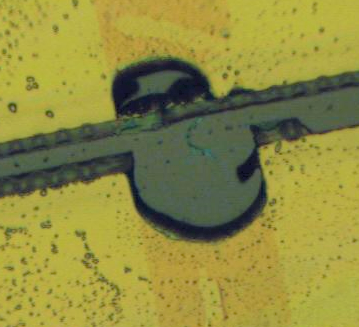
\includegraphics{./figures/ch4/apr-21-dmso-damage.png}

}

}

\subcaption{\label{fig-electrode-dmso-damage}Damage to gold electrode in
channel region after DMSO lift-off}
\end{minipage}%
%
\begin{minipage}[t]{0.05\linewidth}

{\centering 

~

}

\end{minipage}%
%
\begin{minipage}[t]{0.47\linewidth}

{\centering 

\raisebox{-\height}{

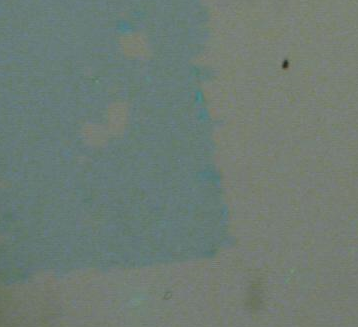
\includegraphics{./figures/ch4/may-21-dmso-damage.png}

}

}

\subcaption{\label{fig-graphene-dmso-damage}Damage to graphene (blue
region) after DMSO lift-off}
\end{minipage}%

\caption{\label{fig-dmso-damage}Lift-off with dimethyl sulfoxide
sometimes led to damage to regions where nanomaterials were present.}

\end{figure}

Dimethyl sulfoxide (DMSO) was sometimes used in lift-off processes
instead of acetone between Jul 2021 and Feb 2023 because of its
effectiveness as a photoresist stripping agent. However, it was
abandoned due to some indications it was too aggressive for the devices
being fabricated, as shown in Figure~\ref{fig-dmso-damage} and also as
detailed in Section~\ref{sec-AFM-characterisation}. It is possible that
heat from the electrodes deposition sometimes crosslinked residual
photoresist on the nanomaterial, and then during lift-off was removed
aggressively together with any attached nanomaterial by the DMSO.
However, it is also possible that prolonged exposure to DMSO alone was
sufficient to detach nanomaterial from the substrate. Therefore, acetone
was the preferred agent for lift-off despite being a less efficient
stripping agent than DMSO.

From Jul 2023 onwards, after each photolithography step, quarter
wafers/chips were flood exposed to UV light for 1 min and then placed in
AZ326 developer for 3 min to ensure complete removal of photoresist
residue (discussed in Section~\ref{sec-fluorescence-characterisation}).

\hypertarget{sec-align}{%
\subsection{Alignment Markers}\label{sec-align}}

Metal alignment markers were deposited in order to accurately align the
device channels with device electrodes in subsequent photolithography
steps. These alignment markers were asymmetric to indicate the
orientation of the device for subsequent photolithography steps and
electrical characteristation. In later discussion, channel 1 is defined
as the channel placed closest to the large, double square alignment
marker.

For carbon nanotube quarter wafers, alignment markers were deposited
either directly before or after carbon nanotube deposition (see
Section~\ref{sec-dep-carbon-nanotubes} for discussion). For graphene
devices, alignment markers were deposited directly after cleaving using
the protective photoresist layer spincoated prior to cleaving.
AZ\(^\circledR\) 1518 was used for alignment marker photolithography.

For carbon nanotube devices made before Jun 2022, chromium was used as
an adhesive layer for gold, while for all graphene devices and carbon
nanotube devices made after Jun 2022, titanium was used as the adhesive
layer. For chromium/gold depositions, a nominal 10 nm of chromium was
deposited followed by a nominal 100 nm Au layer. For titanium/gold
depositions, a nominal 20 nm of titanium was deposited followed by a
nominal 50 nm Au layer (for independent measurements of metal layer
thickness, see Section~\ref{sec-electrodes}). Devices were then soaked
in acetone for at least 2 hours for photoresist lift-off, washed in IPA
and dried with nitrogen. The use of titanium gave rise to a cleaner
lift-off and improved gold adhesion. Using a relatively thin gold layer
(50 nm nominal instead of 100 nm) proved to still be clearly visible but
to a cleaner lift-off.

\hypertarget{channel-etching}{%
\subsection{Channel Etching}\label{channel-etching}}

\begin{figure}

\begin{minipage}[t]{0.47\linewidth}

{\centering 

\raisebox{-\height}{

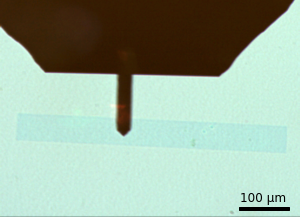
\includegraphics{./figures/ch4/channel-area.png}

}

}

\subcaption{\label{fig-graphene-channel-etch}Graphene channel after
photolithographically defined plasma etch}
\end{minipage}%
%
\begin{minipage}[t]{0.05\linewidth}

{\centering 

~

}

\end{minipage}%
%
\begin{minipage}[t]{0.47\linewidth}

{\centering 

\raisebox{-\height}{

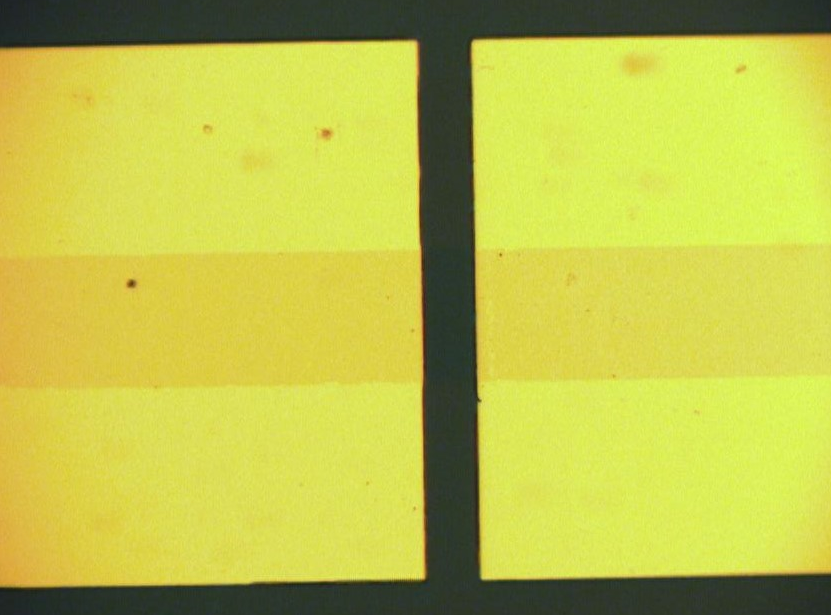
\includegraphics{./figures/ch4/graphene-channel-electrodes.png}

}

}

\subcaption{\label{fig-graphene-channel-electrodes}Graphene channel
after photolithographically defined electrodes deposition and liftoff}
\end{minipage}%

\caption{\label{fig-microscope-graphene-channel}Microscope images of a
graphene channel after plasma etch and electrodes photolithography
steps.}

\end{figure}

Eight channel features, each 1000 \(\mu\)m in length and 100 \(\mu\)m in
width with a pitch of 1200 \(\mu\)m, were patterned using
AZ\(^\circledR\) 1518 photolithography on each carbon nanotube or
graphene-covered substrate. Unwanted nanomaterial not covered with
photoresist was then etched away with 200 W oxygen plasma at 600 mTorr
using a reactive ion etcher or RIE (Plasmalab\(^\circledR\) 80 Plus,
Oxford Instruments). The etch time was 3 minutes for carbon nanotube
quarter wafers, and 1 minute for graphene chips. The protective
photoresist was then removed by soaking in acetone for at least 5
minutes.

\hypertarget{sec-electrodes}{%
\subsection{Electrodes}\label{sec-electrodes}}

The source and drain electrodes for each channel were patterned using
photolithography with either AZ\(^\circledR\) 1518 photoresist (pre-Mar
2023) or AZ\(^\circledR\) nLOF 2020 photoresist (post-Mar 2023). As with
the alignment markers deposition (see Section~\ref{sec-align}), before
Jun 2022 10 nm of chromium was used for the gold adhesive layer, and
after Jun 2022 20 nm of titanium was used. Good electronic contact could
be made with electrodes with a nominal gold layer thickness of 60-100 nm
(see Section~\ref{sec-electrical-characterisation}), and a Au layer
nominally 100 nm thick was most commonly used. Example height profiles
of a chromium sticking layer device and a titanium sticking layer device
taking using a Veeco Dektat 150 profiler are shown in
\textbf{?@fig-dektat-sticking-layer}.

Although AZ\(^\circledR\) nLOF 2020 photolithography was more complex,
it gave rise to more cleanly-defined electrodes with a more consistent
height profile. Using a Veeco Dektat 150 profiler

\hypertarget{encapsulation}{%
\subsection{Encapsulation}\label{encapsulation}}

\hypertarget{photoresist-encapsulation}{%
\subsubsection*{Photoresist
encapsulation}\label{photoresist-encapsulation}}
\addcontentsline{toc}{subsubsection}{Photoresist encapsulation}

\hypertarget{metal-oxide-ceramic-encapsulation}{%
\subsubsection*{Metal oxide (ceramic)
encapsulation}\label{metal-oxide-ceramic-encapsulation}}
\addcontentsline{toc}{subsubsection}{Metal oxide (ceramic)
encapsulation}

\hypertarget{sec-fluorescence-characterisation}{%
\section{Characterisation via Fluorescence
Microscopy}\label{sec-fluorescence-characterisation}}

\hypertarget{sec-AFM-characterisation}{%
\section{Characterisation via Atomic Force
Microscopy}\label{sec-AFM-characterisation}}

\hypertarget{sec-electrical-characterisation}{%
\section{Electrical
Characterisation}\label{sec-electrical-characterisation}}

\bookmarksetup{startatroot}

\hypertarget{functionalisation-of-carbon-nanotubes-and-graphene-with-odorant-receptors}{%
\chapter{Functionalisation of Carbon Nanotubes and Graphene with Odorant
Receptors}\label{functionalisation-of-carbon-nanotubes-and-graphene-with-odorant-receptors}}

\hypertarget{linker-molecules}{%
\section{Linker molecules}\label{linker-molecules}}

\hypertarget{pyrenebutanoic-acid-n-hydroxysuccinimide-ester-pbase}{%
\subsection{1-Pyrenebutanoic acid N-hydroxysuccinimide ester
(PBASE)}\label{pyrenebutanoic-acid-n-hydroxysuccinimide-ester-pbase}}

\begin{figure}

\begin{minipage}[t]{0.47\linewidth}

{\centering 

\raisebox{-\height}{

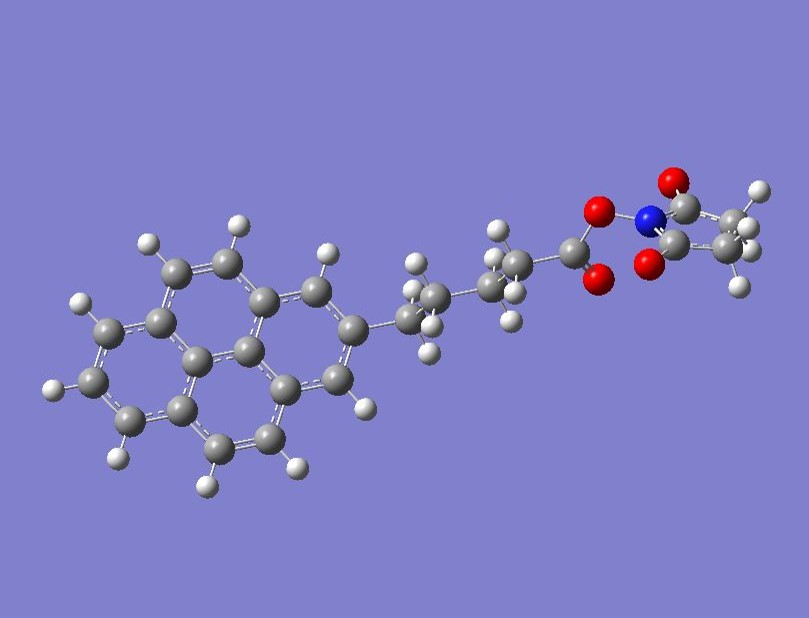
\includegraphics{./figures/ch5/pbase_stable_1.png}

}

}

\subcaption{\label{fig-pbase-stable-1}Hartree-Fock energy: -3427728.67
kJ/mol (9 s.f.)}
\end{minipage}%
%
\begin{minipage}[t]{0.05\linewidth}

{\centering 

~

}

\end{minipage}%
%
\begin{minipage}[t]{0.47\linewidth}

{\centering 

\raisebox{-\height}{

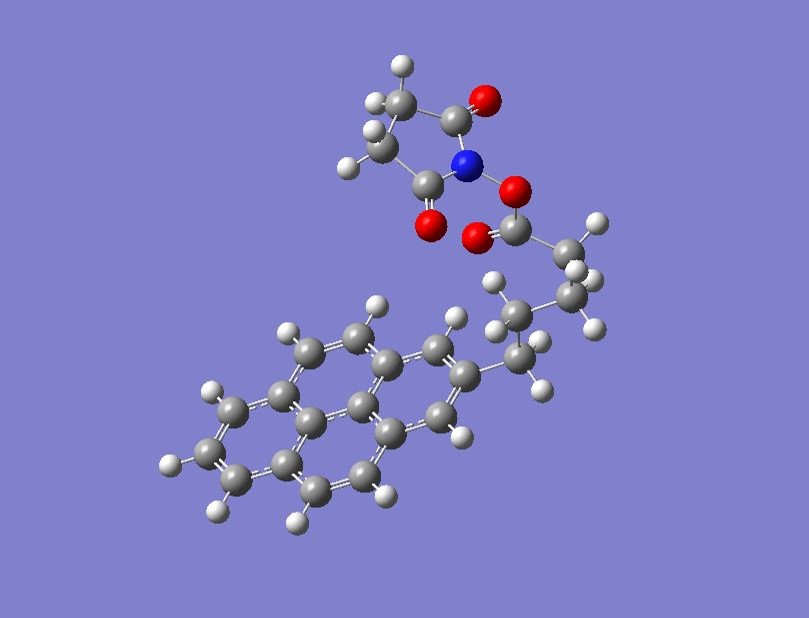
\includegraphics{./figures/ch5/pbase_stable_2.png}

}

}

\subcaption{\label{fig-pbase-stable-2}Hartree-Fock energy: -3427729.66
kJ/mol (9 s.f.)}
\end{minipage}%

\caption{\label{fig-pbase-structure}Two conformations of PBASE molecule
with geometry optimised via \emph{ab initio} calculation (computed using
Gaussian 16 \autocite{g16}). The difference between computed
Hartree-Fock energies is 1.0 kJ/mol, small enough that the existence of
both molecular conformations is physically possible.}

\end{figure}

1-Pyrenebutanoic acid N-hydroxysuccinimide ester (variously known
commercially and in the literature as 1-Pyrenebutyric acid
N-hydroxysuccinimide ester, PBASE, PBSE, PASE, Pyr-NHS, PyBASE, PANHS)
is a aromatic, bifunctional molecule commonly used for tethering
biomolecules to the carbon rings of graphene and carbon nanotubes. The
optimised molecular structure of PBASE is shown in
Figure~\ref{fig-pbase-structure}.

The non-covalent functionalisation of proteins onto a single-walled
carbon nanotube using PBASE was first reported by Chen \emph{et al.} in
2001 \autocite{Chen2001}. Two methods for protein functionalisation and
immobilisation were successfully used, with the only differences being
the solvent used to dissolve the PBASE powder (DMF, methanol) and the
final concentration of the resulting solutions (6 mM, 1 mM
respectively). The lower concentration may have been used for PBASE in
methanol as PBASE powder appears to dissolve poorly in methanol at
higher concentrations. Cella \emph{et al.}, Campos \emph{et al.}, Zheng
\emph{et al.} and Ohno \emph{et al.} all directly cite Chen \emph{et
al.} when discussing functionalisation with PBASE
\autocite{Cella2010,Campos2019,Zheng2016,Ohno2010}. Other groups using
PBASE for graphene or carbon nanotube functionalisation do not
explicitly reference Chen \emph{et al.} in their methodology, but it is
apparent they often draw on one of these two original methods. This
common ancestry becomes apparent from the high frequency of methods
detailing the use of 6 mM PBASE in DMF and 1 mM PBASE in methanol, as
seen in Table~\ref{tbl-pbase-functionalisation}.

However, despite this shared heritage, it is also apparent from
Table~\ref{tbl-pbase-functionalisation} that there is a large degree of
variation in the methods used for PBASE functionalisation. Various
electrical characterisation, microscopy and spectroscopy techniques have
been used to demonstrate successful functionalisation. However, there
has historically been little justification provided for the exact
parameters used in the procedure. As noted by Zhen \emph{et al.} and
Hinnemo \emph{et al.}, there is more generally a lack of systematic
research into formation of pyrene-derivative monolayers on graphene and
other carbon nanomaterials, despite the wide use of this chemistry in
the literature \autocite{Zhen2018,Hinnemo2017}.

\begin{figure}

\begin{minipage}[t]{\linewidth}

{\centering 

\raisebox{-\height}{

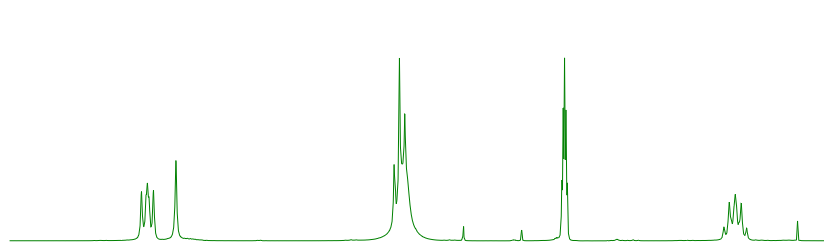
\includegraphics{./figures/ch5/sigma_pbase_nmr.png}

}

}

\subcaption{\label{fig-sigma-nmr}Sigma PBASE in DMSO}
\end{minipage}%
\newline
\begin{minipage}[t]{\linewidth}

{\centering 

\raisebox{-\height}{

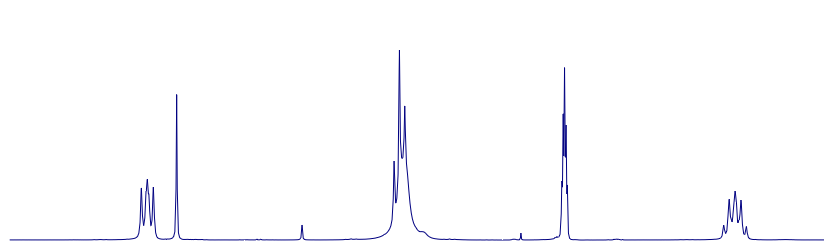
\includegraphics{./figures/ch5/setareh_pbase_nmr.png}

}

}

\subcaption{\label{fig-setareh-nmr}Setareh PBASE in DMSO}
\end{minipage}%
\newline
\begin{minipage}[t]{\linewidth}

{\centering 

\raisebox{-\height}{

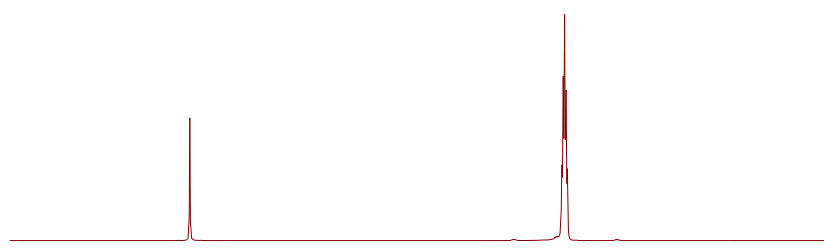
\includegraphics{./figures/ch5/dmso_nmr.png}

}

}

\subcaption{\label{fig-dmso-nmr}Blank (DMSO only)}
\end{minipage}%

\caption{\label{fig-pbase-nmr}Comparison of NMR spectrum profiles
(arbitrary units)}

\end{figure}

We purchased PBASE from two suppliers, Sigma-Aldrich and Setareh
Biotech. Sigma recommends DMF and methanol as suitable solvents for
dissolving PBASE alongside chloroform and DMSO. Setareh Biotech
indicates methanol can be used for dissolving PBASE. The two suppliers
have conflicting information for suitable storage of PBASE, with Sigma
recommending room temperature storage while Setareh Biotech recommends
storage of \(-5\) to \(-30 ^\circ \text{C}\) and protection from light
and moisture. Figure~\ref{fig-pbase-nmr} compares the shapes of NMR
spectra of PBASE from each supplier dissolved in DMSO, alongside a blank
DMSO spectrum.

\newpage
\KOMAoptions{paper=landscape,pagesize}

\hypertarget{tbl-pbase-functionalisation}{}
\begin{longtable}[]{@{}llllrll@{}}
\caption{\label{tbl-pbase-functionalisation}Comparison of PBASE
functionalisation processes used for immobilisation of proteins and
aptamers onto liquid-gated CNTFET and graphene FET
sensors}\tabularnewline
\toprule()
Solvent & Channel & Conc. (mM) & Incubation type & Time (hr) & Rinse
steps & References \\
\midrule()
\endfirsthead
\toprule()
Solvent & Channel & Conc. (mM) & Incubation type & Time (hr) & Rinse
steps & References \\
\midrule()
\endhead
DMF & CNTs & 5 & Immersed & 1 & PBS & Maehashi \textit{et al.}
\cite{Maehashi2007} \\
& & 6 & Immersed & 1 & DMF, PBS & García-Aljaro \textit{et al.}
\cite{Garcia-Aljaro2010} \\
& & 6 & Immersed & 1 & DMF & Chen \textit{et al.} \cite{Chen2001} \\
& & 6 & Immersed & 1 & DMF & Cella \textit{et al.} \cite{Cella2010} \\
& & 6 & Immersed & 1 & DMF & Das \textit{et al.} \cite{Das2011} \\
& Graphene & - & - & 2 & DMF & Kwong Hong Tsang \textit{et al.}
\cite{KwongHongTsang2019} \\
& & - & - & 20 & - & Wiedman \textit{et al.} \cite{Wiedman2017} \\
& & 0.2 & Immersed & 20 & DMF, IPA, DI water & Gao \textit{et al.}
\cite{Gao2018} \\
& & 1 & 100 \(\mu\)L droplet & 6 & DMF, IPA, DI water & Nekrasov
\textit{et al.} \cite{Nekrasov2021} \\
& & 5 & Immersed & 1 & DMF, DI water & Hwang \textit{et al.}
\cite{Hwang2016} \\
& & 6 & 6 \(\mu\)L droplet & 2 & DMF, DI water & Nur Nasufiya
\textit{et al.} \cite{NurNasyifa2020} \\
& & 10 & 10 \(\mu\)L droplet & 2 & DMF, DI water & Campos
\textit{et al.} \cite{Campos2019} \\
& & 10 & Immersed & 2 & DMF, PBS & Kuscu \textit{et al.}
\cite{Kuscu2020} \\
& & 10 & Immersed & 1 & DMF & Xu \textit{et al.} \cite{Xu2017} \\
& & 10 & Immersed & 12 & DMF, ethanol, DI water & Khan \textit{et al.}
\cite{Khan2020} \\
2-Methoxyethanol & Graphene & 1 & Immersed & 1 & DI water & Ono
\textit{et al.} \cite{Ono2020} \\
Methanol & CNTs & 1 & Immersed & 1 & Methanol, DI water & Zheng
\textit{et al.} \cite{Zheng2016} \\
& & 1 & Immersed & 2 & Methanol & Kim \textit{et al.} \cite{Kim2009} \\
& Graphene & 5 & Immersed & 2 & - & Sethi \textit{et al.}
\cite{Sethi2020} \\
& & 5 & Immersed & 1 & Methanol, PBS & Ohno \textit{et al.}
\cite{Ohno2010} \\
DMSO & CNTs & 10 & - & 1 & DI water & Lopez \textit{et al.}
\cite{Lopez2015} \\
& & 10 & Immersed & 1 & PBS & Strack \textit{et al.}
\cite{Strack2013} \\
\bottomrule()
\end{longtable}

\newpage
\KOMAoptions{paper=portrait,pagesize}

\bookmarksetup{startatroot}

\hypertarget{results}{%
\chapter{Results}\label{results}}

What I found out.

See for more detailed results

\bookmarksetup{startatroot}

\hypertarget{vapour-phase-sensing-with-transistor-biosensors}{%
\chapter{Vapour Phase Sensing with Transistor
Biosensors}\label{vapour-phase-sensing-with-transistor-biosensors}}

\hypertarget{testing-vapour-delivery-system}{%
\section{Testing Vapour Delivery
System}\label{testing-vapour-delivery-system}}

\hypertarget{system-description}{%
\subsection{System Description}\label{system-description}}

\begin{figure}

{\centering 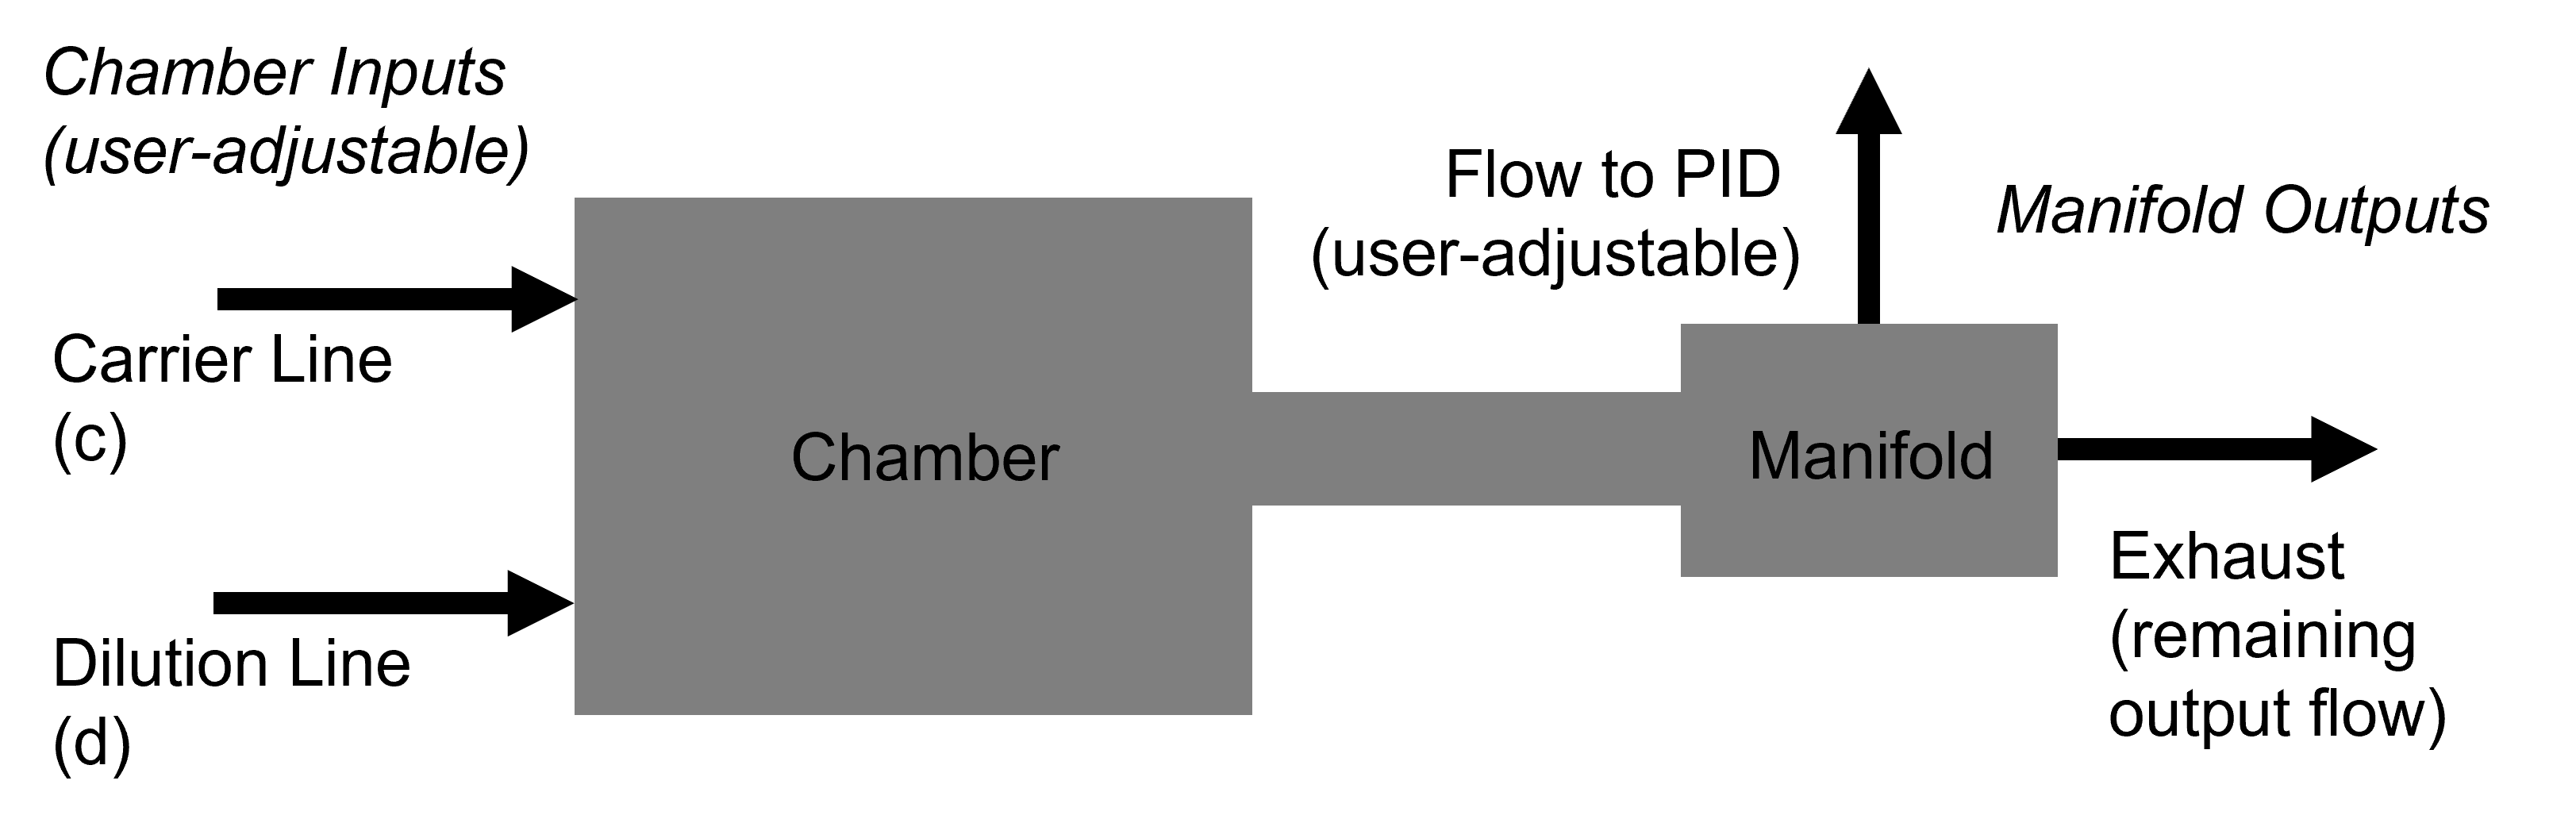
\includegraphics[width=0.9\textwidth,height=\textheight]{./figures/ch7/chamber-manifold.png}

}

\caption{Vapour Delivery System - Schematic of device chamber and
manifold}

\end{figure}

\hypertarget{temperature-and-humidity-indicator}{%
\subsection{Temperature and Humidity
Indicator}\label{temperature-and-humidity-indicator}}

\hypertarget{photoionisation-detector}{%
\subsection{Photoionisation Detector}\label{photoionisation-detector}}

\hypertarget{bubbling-vapour}{%
\subsubsection*{Bubbling Vapour}\label{bubbling-vapour}}
\addcontentsline{toc}{subsubsection}{Bubbling Vapour}

First year report: ``\,````First, a 200 sccm flow of N2 gas was sent
through the dilution line to the device chamber until 1000 s. Then, the
flow controller three-way valves were manually adjusted so that the same
200 sccm flow was directed through 50 mL of EtOH analyte in the carrier
line. This continued until 2200 s, where the valves were again manually
adjusted so that 200 sccm clean N2 again flowed through the device
chamber. The resulting current across the device channel was monitored
over this time, and is shown in Figure 19. A response to EtOH exposure
and removal is visible.''``\,''

\bookmarksetup{startatroot}

\hypertarget{summary}{%
\chapter{Summary}\label{summary}}

In summary, this book has no content whatsoever.

\begin{verbatim}
[1] 2
\end{verbatim}

\appendix
\addcontentsline{toc}{part}{Appendices}

\hypertarget{sec-photolithography}{%
\chapter{Photolithography}\label{sec-photolithography}}

\begin{figure}

{\centering 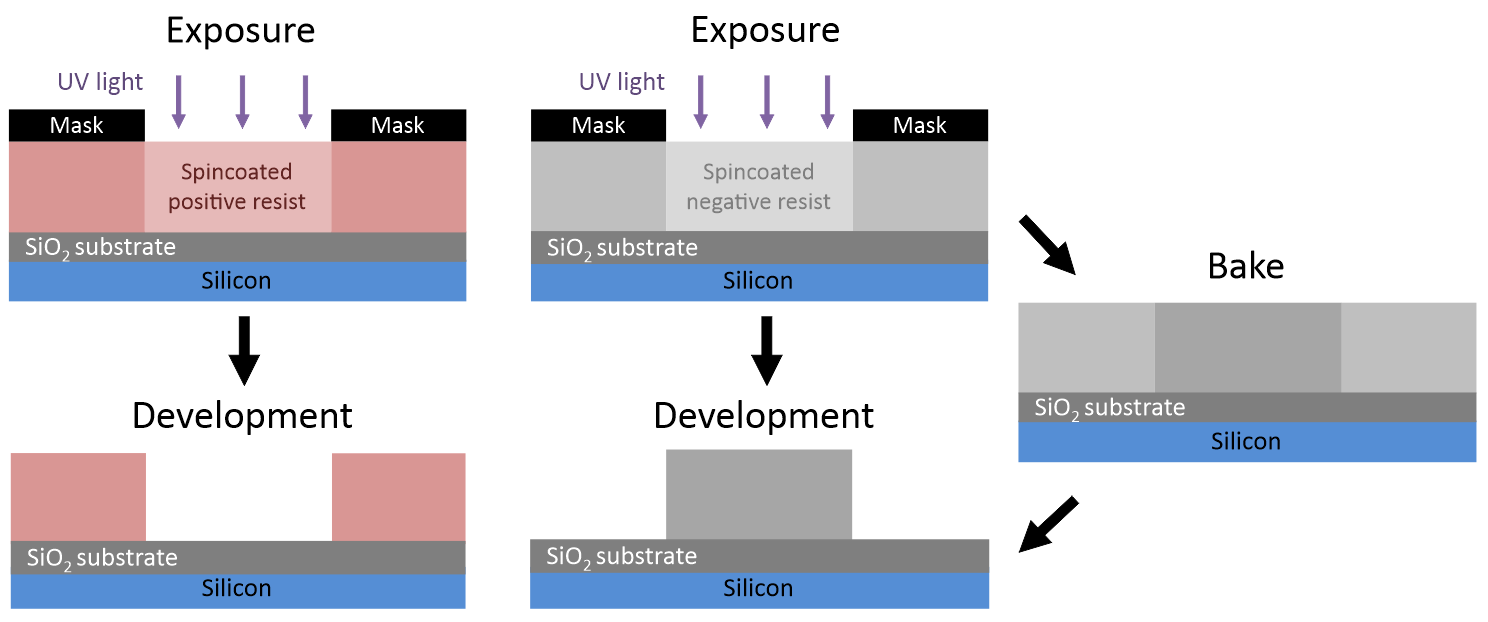
\includegraphics{./figures/app1/positive-negative-photolithography.png}

}

\caption{\label{fig-photolithography-types}A side-view comparison of
generic photolithography processes for positive and negative resists in
the ideal case. Photolithography with a positive resist requires a
single softbake step before exposure, while for negative resists a
second baking step is required after exposure (Thicknesses shown not to
scale).}

\end{figure}

This section details some of the standard photolithography procedures
used in the device fabrication processes detailed in
Chapter~\ref{sec-fabrication}. Photoresists, also referred to here as
``resists'', are UV light-sensitive polymeric resins used for
photolithography. Both positive and negative photoresists were used in
various fabrication processes. Positive resists are made soluble in
alkalines by UV light exposure, meaning exposed areas are removed in the
development process. Conversely, negative resists are cross-linked by
exposure and a post-exposure bake step. The unexposed areas of the
negative resist are then removed in the development process
\autocite{Microchemicals}. Figure~\ref{fig-photolithography-types} gives
a visual representation of these differences.

\begin{figure}

\begin{minipage}[t]{0.47\linewidth}

{\centering 

\raisebox{-\height}{

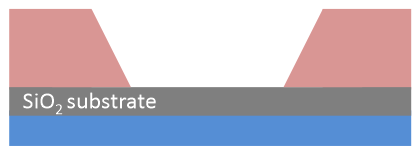
\includegraphics{./figures/app1/overcut-profile.png}

}

}

\subcaption{\label{fig-overcut-profile}Overcut profile of a positive
resist}
\end{minipage}%
%
\begin{minipage}[t]{0.05\linewidth}

{\centering 

~

}

\end{minipage}%
%
\begin{minipage}[t]{0.47\linewidth}

{\centering 

\raisebox{-\height}{

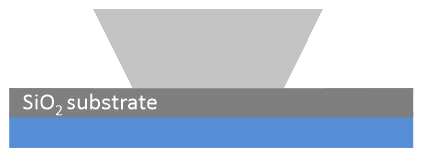
\includegraphics{./figures/app1/undercut-profile.png}

}

}

\subcaption{\label{fig-undercut-profile}Undercut profile of a negative
resist}
\end{minipage}%

\caption{\label{fig-photolithography-profiles}Two different resist
profiles seen for different types of photoresist. The undercut profile
is ideal for thin-film metal deposition and subsequent patterned
removal, known as ``lift-off''.}

\end{figure}

The specific photoresist selected for photolithography depends on the
specific use case. The types used in this thesis are positive and
negative AZ\(^\circledR\) photoresists (AZ\(^\circledR\) 1518,
Microchemicals GmbH; AZ\(^\circledR\) nLOF 2020, Microchemicals GmbH)
and SU-8 (SU8-2150, Kayaku Advanced Materials, formerly Microchem). The
AZ\(^\circledR\) resists used here have a minimum film thickness of
\(1.5\textrm{ } \mu \textrm{m}\) \autocite{Microchemicals}, while the
SU8-2150 has a minimum film thickness of
\(0.5\textrm{ } \mu \textrm{m}\) \autocite{Kayaku}. Positive resists
which have not been thermally crosslinked will soften at higher
temperatures (\(\gtrsim 100^\circ\)C for AZ\(^\circledR\) 1518), leading
to a rounded profile. This is not the case for negative resists, which
are more thermally stable \autocite{Microchemicals}. Each resist
therefore has a different cross-section profile, as shown in
Figure~\ref{fig-photolithography-profiles}.

The negative resist profile is more suited to metal or metal oxide
deposition and lift-off processes \autocite{Microchemicals}, though the
process is more sensitive to error due to the extrarequiring more
processing steps than positive resist. Finally, when it is suitably
processed SU-8 is considered to be more biocompatible than other
photoresists. It is especially biocompatible when chemically modified
via processes such as isopropanol sonication and O\(_2\) plasma
treatment \autocite{Chen2021}.

All photolithographic exposure was performed on a Karl Suss MJB3 Contact
Aligner with a USHIO super-high pressure 350 W mercury lamp (USH-350DS,
Japan). When performing lithography, the intensity reading from the
aligner was 20.8 - 24.2 mW/cm\(^2\) (Note however that an external
photometer reading at 400 nm found an intensity output of 17.2
mW/cm\(^2\) when the aligner read 21.0 mW/cm\(^2\)).

In general, photolithography procedures should be performed under yellow
lighting, as light wavelengths from 320-450 nm can promote reactions in
the photoresist used. Aging of photoresist over time can also
significantly affect the photolithography process, and therefore all
processes should be re-optimised regularly over time to give the desired
result \autocite{Microchemicals}. The range in processing times for some
steps of the processes used here are largely due to the effects of aging
on the photoresist.

The step-by-step processes for each resist are detailed in the
subsequent sections.

\hypertarget{azcircledr-1518-photoresist}{%
\section{\texorpdfstring{AZ\(^\circledR\) 1518
photoresist}{AZ\^{}\textbackslash circledR 1518 photoresist}}\label{azcircledr-1518-photoresist}}

\begin{enumerate}
\def\labelenumi{\arabic{enumi}.}
\item
  Spincoat at a final speed of 4000 rotations per minute (rpm) for 1
  minute, with an initial acceleration of 500 rpm/s (notes: clean the
  substrate with acetone, isopropanol (IPA) and nitrogen before
  spincoating; use only the minimum amount of photoresist required to
  fully cover the wafer surface; avoid any gaps or bubbles in the
  photoresist).
\item
  Softbake 2-4 minutes at \(95^\circ\)C on the hotplate (2 min for
  individual devices, 4 min for a quarter wafer)
\item
  Mask expose for 10-12 s (note: clean mask with acetone/IPA and N\(_2\)
  dry before use)
\item
  Develop with 3 parts AZ\(^\circledR\) 326 (2.38 \% TMAH metal-ion free
  developer, Microchemicals GmbH) in 1 part deionised (DI) water for
  30-45 s (note: rinse for 10-15 s in one development solution, then
  perform the rest of the development in clean developer for a cleaner
  profile)
\item
  Rinse device for 30 s in DI water to remove excess developer, then dry
  under nitrogen
\end{enumerate}

\hypertarget{azcircledr-nlof-2020-photoresist}{%
\section{\texorpdfstring{AZ\(^\circledR\) nLOF 2020
photoresist}{AZ\^{}\textbackslash circledR nLOF 2020 photoresist}}\label{azcircledr-nlof-2020-photoresist}}

\begin{enumerate}
\def\labelenumi{\arabic{enumi}.}
\item
  Spincoat at final speed of 3000 rotations per minute (rpm) for 1
  minute, with an initial acceleration of 500 rpm/s (notes: clean the
  substrate with acetone, isopropanol (IPA) and nitrogen before
  spincoating; avoid any gaps or bubbles in the photoresist)
\item
  Softbake for precisely 60 s at \(110^\circ\)C on the hotplate
\item
  Mask expose for 2.7-3 s (note: clean mask with acetone/IPA and N\(_2\)
  dry before use)
\item
  Post-exposure bake for precisely 60 s at \(110^\circ\)C on the
  hotplate to cross-link exposed resist
\item
  Develop with 3 parts AZ\(^\circledR\) 326 in 1 part DI water for 60-70
  s (note: rinse for 30 s in one development solution, then perform the
  rest of the development in clean developer for a cleaner profile)
\item
  Rinse device for 30 s in DI water to remove excess developer, then dry
  under nitrogen
\end{enumerate}

\hypertarget{su8-2150-photoresist}{%
\section{SU8-2150 photoresist}\label{su8-2150-photoresist}}

\begin{enumerate}
\def\labelenumi{\arabic{enumi}.}
\item
  SU-8 was diluted in cyclopentanone until viscosity was low enough to
  spincoat on substrate and then sonicated at \(50^\circ\)C for 3-4
  hours (Note: The dilution ratio used was \textasciitilde1 part SU-8 to
  5 parts cyclopentanone. However, the age of the SU-8 may mean that
  significant evaporation had occurred prior to use, and the amount of
  SU-8 actually present is underrepresented by this ratio)
\item
  Spincoat first with a final speed of 500 rpm (acceleration 500 rpm/s)
  for 10 seconds, followed by spincoating at 4000 rpm (acceleration 7500
  rpm/s) for 40 s.
\item
  Softbake for 10 minutes at \(95^\circ\)C on the hotplate
\item
  Mask expose for 6-8 s (note: clean mask with acetone/IPA and N\(_2\)
  dry before use)
\item
  Post-exposure bake for 10 minutes at \(95^\circ\)C on the hotplate to
  cross-link exposed resist
\item
  Develop with SU-8 developer (Kayaku Advanced Materials, formerly
  Microchem) for 10-15 s, then clean in IPA for 30 s, repeat this step
  once then dry under nitrogen
\end{enumerate}

\hypertarget{sec-python}{%
\chapter{Python Code for Data Analysis}\label{sec-python}}

\hypertarget{vapour-delivery-system}{%
\chapter{Vapour Delivery System}\label{vapour-delivery-system}}

\hypertarget{technical-notes}{%
\section{Technical Notes}\label{technical-notes}}

Two LabView Virtual Instruments (VIs) were adapted from pre-existing VIs
for operating the mass flow controllers and monitoring vapour flow into
the device chamber, as well as monitoring temperature and humidity in
the vapour delivery system's manifold. These VIs were named ``\,'' A
third VI was developed in parallel which combined the first two Virtual
Instruments, alongside allowing the sequence of values to control the
mass flow controllers.

From Honours report: ``\,``\,'' Figure 12 gives the right side of the
front panel of the LabView VI sample with vapour.VI, which letsus preset
an autonomously-performed vapour sensing sequence. Each row in each
array module corresponds to a differennest step in this sequence. The
`howManySteps' module lets us set how many of these steps are performed.
The `Durations Array' module determines the length of time in seconds
each step is performed over. The `Carrier Flows Array' and `Dilution
Flows Array' modules let us set the carrier flow and dilution flow,
respectively, in standard cubic centimetres per minute (sccm) through
the gas rig at each step. The carrier flow pushes analyte vapour into
the vapour-sensing device chamber, while dilution flow is used to modify
the flow behaviour of the analyte vapour entering the chamber. The
vapour sensing sequence as depicted in Figure 12 was used for all vapour
sensing runs in this investigation. At the end of the sequence, the data
collected about the vapour sensing process was saved as an .lvm file.
``\,``\,''

\hypertarget{future-improvements}{%
\section{Future Improvements}\label{future-improvements}}


\backmatter
\printbibliography


\end{document}
